\begin{figure}[t]
    \centering
    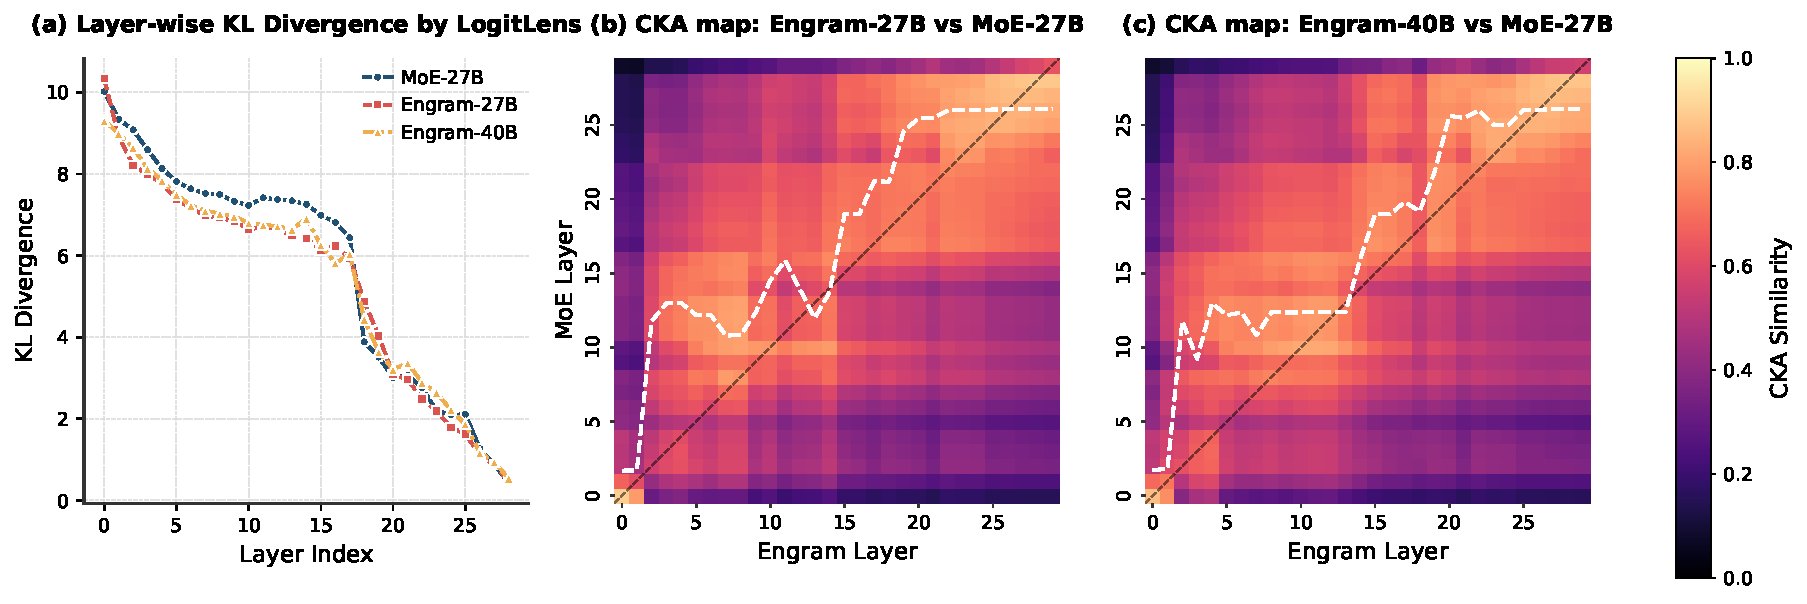
\includegraphics[width=\linewidth]{figs/logitlens_and_cka.pdf}
    \caption{\textbf{Analysis of representational alignment and convergence speed.} (a) Layer-wise KL Divergence via LogitLens~\citep{nostalgebraist2020logitlens}. The consistently lower divergence in early layers indicates that Engram accelerates prediction convergence. (b-c) Similarity heatmap computed by CKA~\citep{kornblith2019similarity}. The distinct upward shift of the high-similarity diagonal demonstrates that =Engram's shallow layers are functionally equivalent to deeper layers of the MoE model, effectively increasing the model's depth.}
    \label{fig:logitlens_and_cka}
\end{figure}


\begin{table}[htbp]
    \centering
    \small
    \renewcommand{\arraystretch}{1.4}
    \caption{
    \textbf{Entity resolution example reproduced from} \citet{ghandeharioun2024patchscopes}. 
    This table illustrates how LLMs gradually integrate context tokens through layers of attention and FFNs to construct the internal representation of the entity: \texttt{``Diana, Princess of Wales''}. The ``Latent State Translation'' column displays the automatically generated text for the last token: \texttt{``Wales''} by PatchScope~\citep{ghandeharioun2024patchscopes}, while the ``Explanation'' column presents the manual interpretation provided by the original authors.
    }

    \begin{tabularx}{0.85\textwidth}{ 
        c 
        >{\RaggedRight\arraybackslash}X 
        >{\RaggedRight\arraybackslash}m{4.5cm} 
    }
        \toprule
        \textbf{Layer} & \textbf{Latent State Translation} & \textbf{Explanation} \\
        \midrule
        
        1-2 &
        : Country in the United Kingdom &
        \textbf{Wales} \\
        
        3 &
        : Country in Europe &
        \textbf{Wales} \\
        
        4 &
        : Title held by female sovereigns in their own right or by queens consort &
        \textbf{Princess of Wales} \newline (unspecific) \\
        
        5 &
        : Title given to the wife of the Prince of Wales (and later King) &
        \textbf{Princess of Wales} \newline (unspecific) \\
        
        6 &
        : Diana, Princess of Wales (1961-1997), the first wife of Prince Charles, Prince of Wales, who was famous for her beauty and humanitarian work &
        \textbf{Diana, \newline Princess of Wales} \\
        \bottomrule
    \end{tabularx}
    \label{tab:patchscope}
\end{table}

\section{Analysis}
In this section, we investigate the internal mechanisms of Engram, including its effective depth~(\autoref{sec:depth_analysis}), core module design~(\autoref{sec:ablation_structural}), and parametric sensitivity~(\autoref{sec:dse_sensitive}). Additionally, we evaluate the inference throughput with offloading~(\autoref{sec:inference_analysis}) and conclude with a case study~(\autoref{sec:case_study}).

\subsection{Is Engram functionally equivalent to increasing the model’s depth?}
\label{sec:depth_analysis}

Current LLMs lack a dedicated knowledge lookup primitive and they rely on computation to simulate memory recall. As shown in \autoref{tab:patchscope}, to recognize the entity $\texttt{"Diana,\,Princess\;of\;Wales"}$, an LLM must consume multiple layers of Attention and FFNs to progressively compose features~\citep{li2025echoesbertmodernlanguage,ghandeharioun2024patchscopes,DBLP:conf/coling/JinYHZWH0MMDYDZ25}, a process that could theoretically be identified via a knowledge lookup operation.

Given this, we posit that by equipping the model with an explicit knowledge lookup capability, Engram effectively mimics an increase in model depth by relieving the model of the early stages of feature composition. To validate this hypothesis, we employ two mechanistic interpretability tools: LogitLens~\citep{nostalgebraist2020logitlens,belrose2023eliciting} and Centered Kernel Alignment analysis (CKA)~\citep{kornblith2019similarity,davari2022reliability}.

\subsubsection{Accelerated Prediction Convergence}
\label{sec:logitlens}

We first analyze the evolution of predictions across layers using LogitLens~\citep{nostalgebraist2020logitlens}. By projecting each intermediate layer's hidden state with the final LM Head, we compute the Kullback–Leibler divergence~\citep{kullback1951information} between the intermediate output distribution and the model's final output distribution. This metric quantifies how close a latent representation is to being ``prediction-ready''~\citep{csordas2025language,belrose2023eliciting}.

\autoref{fig:logitlens_and_cka} (a) reports the layer-wise KL divergence. Compared to the MoE baseline, both Engram variants exhibit systematically smaller KL divergence, with the most pronounced gap appearing in the early blocks. The steeper descent in the Engram curves indicates that the model finishes feature composition much faster. This observation aligns with our hypothesis: by accessing external knowledge explicitly, Engram reduces the computational steps required, thereby reaching high-confidence, valid predictions earlier in the network hierarchy.

\subsubsection{Representational Alignment and Effective Depth}

To further investigate whether Engram layers semantically correspond to deeper layers of the baseline, we employ Centered Kernel Alignment~(CKA), a widely established metric for comparing representational structures~\citep{kornblith2019similarity,kriegeskorte2008representational}. Given two sets of representations $X$ and $Y$ (e.g., activations from different models or layers), CKA is defined as:
\begin{equation}
    \text{CKA}(K, L) = \frac{\text{HSIC}(K, L)}{\sqrt{\text{HSIC}(K, K)\text{HSIC}(L, L)}}
\end{equation}
where $K = XX^\top$ and $L = YY^\top$ denote the Gram matrices (using a linear kernel) and HSIC is Hilbert-Schmidt Independence Criterion~\citep{gretton2005measuring}. We employ a minibatch implementation with an unbiased estimator of HSIC~\citep{davari2022reliability} and evaluate on the Few-NERD dataset~\citep{ding2021few}, extracting hidden states corresponding to the final token of named entities.

To rigorously quantify the layer-wise correspondence, 
we first compute the pairwise CKA similarity matrix $S \in [0, 1]^{L \times L}$, where $L$ is the number of layers. We then introduce a soft alignment index $a_j$, defined as the weighted centroid of the top-$k$ most similar MoE layers for each Engram layer $j$:
\begin{equation}
    a_j = \frac{\sum_{i \in \mathcal{I}_j} S_{i,j} \cdot i}{\sum_{i \in \mathcal{I}_j} S_{i,j}}, \quad \text{where } \mathcal{I}_j = \mathop{\text{argtop}k}_{i} (S_{i,j}). 
\end{equation}
Here, $S_{i,j}$ denotes the similarity score between MoE layer $i$ and Engram layer $j$. The index $a_j$ serves as a robust proxy for the ``effective MoE depth'' corresponding to Engram layer $j$, utilizing top-$k$ filtering (with $k=5$) to mitigate low-similarity noise.

\autoref{fig:logitlens_and_cka} (b)--(c) visualize the similarity heatmaps overlayed with the soft alignment curve (dashed white line). We observe a distinct upward shift from the diagonal, meaning that $a_j > j$ for a wide range of layers. For instance, the representations formed at layer 5 of Engram-27B align most closely with those at approximately layer 12 of the MoE baseline.

The consistent off-diagonal shift, which aligns with the LogitLens results~(\autoref{sec:logitlens}), confirms that Engram achieves deeper representations at earlier layers. This validates our central hypothesis: by bypassing early-stage feature composition via explicit lookups, Engram is functionally equivalent to increasing the model's effective depth.

\begin{figure}[t]
\centering
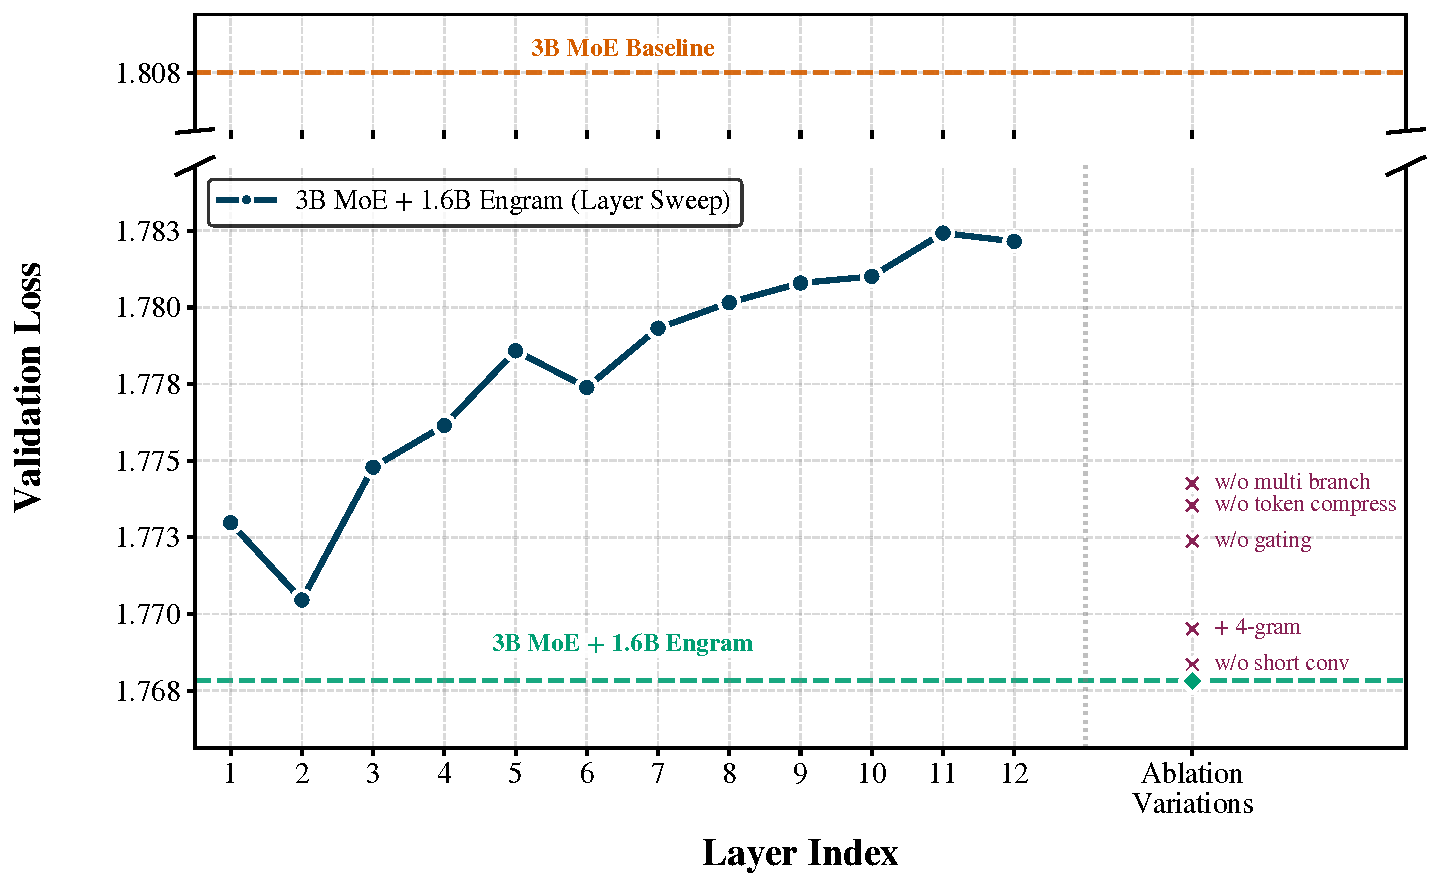
\includegraphics[width=0.75\linewidth]{figs/arch_ablation.pdf}
\caption{
    \textbf{Architecture ablation results.}
    We compare the 3B MoE baseline against Engram variations in two settings:
    (1) Layer Sensitivity (dark blue curve): Sweeping the insertion depth of a single Engram module confirms that early injection (Layer 2) is optimal, whereas efficacy degrades in deeper layers.
    (2) Component Ablation (Right Markers): Removing sub-modules from the reference configuration demonstrates the importance of multi-branch integration, tokenizer compression, and context-aware gating.
}
\label{fig:arch_ablation}
\end{figure}

\subsection{Structural Ablation and Layer Sensitivity}
\label{sec:ablation_structural}

In this section, we ablate Engram under a controlled setting to investigate the effectiveness of each key module design.
Unless otherwise specified, the backbone is a 12-layer 3B MoE model (0.56B activated parameters) trained for 100B tokens.
\autoref{fig:arch_ablation} reports validation loss.
The dashed orange line denotes the 3B MoE baseline (Val Loss $=1.808$).

\paragraph{Reference configuration.}
We augment the backbone with a fixed 1.6B-parameter Engram memory.
Our reference model uses $\{2,3\}$-grams and inserts Engram at Layers 2 and 6, achieving Val Loss $=1.768$,
a substantial improvement over the MoE baseline ($\Delta=0.04$).
All structural ablations below are defined relative to this reference.

\paragraph{Where should memory be injected?}
To study depth sensitivity, we keep the Engram budget fixed (1.6B) but consolidate it into a single Engram module,
and sweep its insertion layer from 1 to 12 (dark blue ``Layer Sweep'' curve in \autoref{fig:arch_ablation}).
This experiment exposes an inherent trade-off in Engram placement.

\textbf{A placement trade-off.}
Injecting Engram early allows it to offload local pattern reconstruction before the backbone expends computational depth, aligning with the backbone's natural hierarchical processing~\citep{tenney2019bert,ghandeharioun2024patchscopes,li2025echoesbertmodernlanguage,DBLP:conf/coling/JinYHZWH0MMDYDZ25}.
However, this incurs a cost in gating precision: early hidden states have not yet aggregated sufficient global context via attention, and the parallel branches lack the representational divergence required for fine-grained modulation~\citep{xie2025mhcmanifoldconstrainedhyperconnections,zhu2025hyperconnections}.
Consequently, optimal placement requires balancing (i) offloading static local patterns early and (ii) utilizing stronger contextual queries for gating later.

The sweep shows that Layer 2 achieves the best single-layer performance (Val Loss $= 1.770$), outperforming Layer 1 and
degrading as the insertion point moves deeper.
This indicates that one round of attention is already sufficient to provide a meaningfully contextualized $\mathbf{h}_t$ for gating,
while still being early enough to replace the backbone's bottom-layer local aggregation.

While Layer 2 is optimal under a single injection constraint, we find that dividing the same 1.6B memory into two smaller
modules (achieved by reducing the embedding dimension $d_{\text{mem}}$) and placing them at Layers 2 and 6 performs even better (Val Loss $=1.768$).
This layered design reconciles the trade-off by combining early intervention with rich, late-stage contextual gating.
More importantly, layered insertion also provides a practical system advantage, enabling better utilization of the memory hierarchy as discussed in \autoref{sec:system_efficiency}.

\paragraph{Which components matter?}
Starting from the reference configuration, we ablate individual design choices while
keeping the Engram parameter budget fixed. Results are denoted by markers in \autoref{fig:arch_ablation}.
We find that three components yield the most significant gains:
(i) branch-specific fusion within the multi-branch backbone,
(ii) context-aware gating, and
(iii) tokenizer compression.
Removing any of these causes the largest regressions in validation loss.
Specifically, for the ``w/o multi branch'' ablation, we retain the mHC backbone structure but replace the branch-specific gating with a single Engram fusion applied to the hidden states after the pre-mapping $\mathcal{H}^{pre}$~\citep{xie2025mhcmanifoldconstrainedhyperconnections}.

Other changes have smaller effects: removing the lightweight depthwise convolution only marginally degrades performance.
Allocating capacity to 4-grams is slightly suboptimal under a fixed 1.6B budget—likely because it dilutes capacity
from the more frequent 2/3-gram patterns—though we do not rule out that higher-order $N$-grams become beneficial at larger memory scales.

\subsection{Sensitivity Analysis}
\label{sec:dse_sensitive}

\begin{figure}[t]
\centering
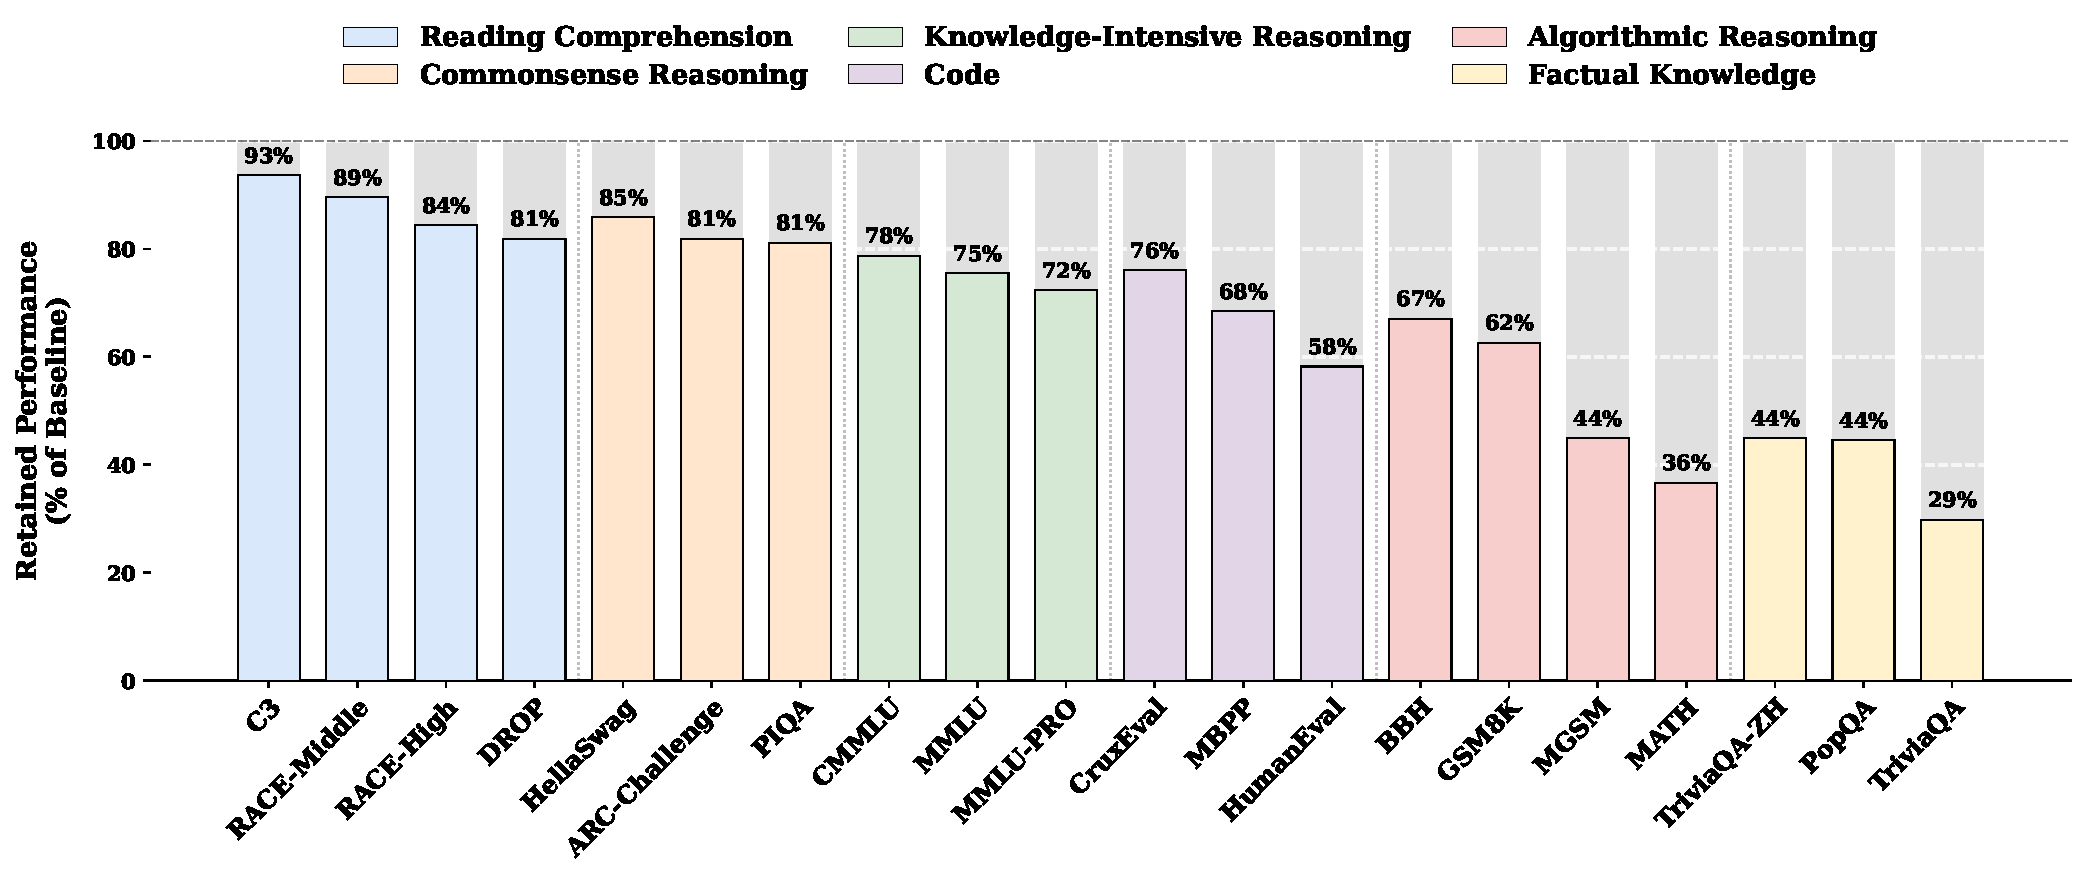
\includegraphics[width=0.9\linewidth]{figs/sensitivity_analysis.pdf}
\caption{\textbf{Retained performance under Engram ablation.} Factual knowledge relies heavily on the Engram module, whereas reading comprehension is largely preserved by the backbone.}
\label{fig:sensitivity_analysis}
\end{figure}



To characterize the functional contribution of the Engram module, we evaluate the model by completely suppressing the sparse embedding output during inference while keeping the backbone unchanged. Crucially, this post-hoc ablation induces a \textbf{training--inference inconsistency}, potentially introducing noise in complex, mixed-capability tasks. Consequently, we prioritize the analysis of \textit{Factual Knowledge} and \textit{Reading Comprehension}—the two extremes of the sensitivity spectrum—which exhibit the highest signal-to-noise ratio under this stress test. 

As shown in \autoref{fig:sensitivity_analysis}, the results reveal a sharp functional dichotomy. Factual knowledge benchmarks suffer a catastrophic collapse, retaining only 29--44\% of the original performance (e.g., TriviaQA at 29\%), confirming that the Engram module acts as the primary repository for parametric knowledge. Conversely, reading comprehension tasks are remarkably resilient, retaining 81--93\% (e.g., C3 at 93\%), suggesting that context-grounded tasks rely primarily on the backbone's attention mechanism rather than Engram.

\subsection{System Efficiency}
\label{sec:inference_analysis}

A pivotal system advantage of Engram over routing-based MoE is that its sparse activations are addressed by explicit, static hash IDs. This yields a strictly deterministic memory access pattern: indices for the next Engram lookup are fixed once the token sequence is known and can be computed before the corresponding layer executes. 

\paragraph{Experimental Setup.}
We implemented an inference harness based on nano-vLLM\footnote{\url{https://github.com/GeeeekExplorer/nano-vllm}}—a streamlined prototype of the industry-standard vLLM engine~\citep{kwon2023efficient}. To obtain a clean latency baseline without the confounding communication patterns of Expert Parallel in MoE, we benchmark on two dense backbones (Dense-4B and Dense-8B).
We insert a massive 100B-parameter Engram layer into the second Transformer block, with the entire embedding table resident in host DRAM.
During inference, the system prefetches embeddings for the Engram layer asynchronously, overlapping the PCIe transfer with the computation of the first block.

\begin{table}[htbp]
    \centering
    \caption{\textbf{End-to-end Inference Throughput}. We measure infernece throughput with a 100B-parameter Engram layer entirely offloaded to host memory.}
    \label{tab:vllm}
    \vspace{2mm}
    \begin{tabular}{llc}
        \toprule
        \multicolumn{3}{c}{\textbf{Experimental Setup}} \\
        \midrule
        \multicolumn{2}{l}{\textit{Hardware}} & NVIDIA H800 \\
        \multicolumn{2}{l}{\textit{Workload}} & 512 Sequences \\
        \multicolumn{2}{l}{\textit{Sequence Length}} & Uniform$(100, 1024)$ \\
        \midrule
        \multicolumn{3}{c}{\textbf{Throughput Results}} \\
        \midrule
        \textbf{Base Model} & \textbf{Configuration} & \textbf{Throughput (tok/s)} \\
        \midrule
        \multirow{2}{*}{4B-Dense} 
            & Baseline & 9,031.62 \\
            & + 100B Engram (CPU Offload) & 8,858.28 \\
        \midrule
        \multirow{2}{*}{8B-Dense} 
            & Baseline & 6,315.52 \\
            & + 100B Engram (CPU Offload) & 6,140.02 \\
        \bottomrule
    \end{tabular}
\end{table}


\paragraph{Results.}
As detailed in \autoref{tab:vllm}, offloading a 100B-parameter embedding table incurs a negligible throughput penalty, peaking at only $2.8\%$ on the 8B backbone.
This confirms that the compute intensity of early dense blocks provides a sufficient temporal window to mask the retrieval latency. Crucially, the effective communication volume per step scales with the number of activated slots rather than the total embedding table size.

Crucially, this experiment serves as a conservative baseline. While the hierarchical design in \autoref{sec:system_efficiency} exploits Zipfian locality to cache frequent items in HBM, our experimental setup forces \textit{all} retrievals to traverse the PCIe bus from host memory. The fact that this baseline retrieval strategy yields minimal overhead strongly suggests that a fully optimized, locality-aware implementation would incur negligible throughput penalty.


\subsection{Case Study: Gating Visualization}
\label{sec:case_study}

In \autoref{sec:engram_fusion}, we introduced the context-aware gating mechanism, designed to dynamically modulate the integration of retrieved static memory into the backbone. To empirically validate whether Engram behaves as intended, we visualize the gating scalar $\alpha_t$ of Engram-27B\footnote{As detailed in our architecture setup, this model utilizes a mHC ($M=4$) with Engram modules inserted at layers 2 and 15. Consequently, for any given token, the model computes a total of 8 distinct gating scalars. We observe that not every branch encodes interpretable activation patterns. For the clarity of this visualization, we select and display the gating values most strongly correlated with semantic pattern matching.} across various samples in \autoref{fig:visualization}.

The results demonstrate a distinct pattern of selectivity. The gating mechanism consistently activates (shown in red) upon completing local, static patterns. In English, we observe strong activations on multi-token named entities (e.g., ``Alexander the Great'', ``the Milky Way'') and formulaic phrases (e.g., ``By the way'', ``Princess of Wales''). This behavior generalizes effectively across languages. In the Chinese examples, Engram identifies and retrieves distinct idiomatic expressions and historical entities, such as ``Four Great Inventions'' (\textbf{四大发明}) and ``Zhang Zhongjing'' (\textbf{张仲景}). These qualitative results confirm that Engram successfully identifies and handles stereotyped linguistic dependencies, effectively relieving the Transformer backbone from memorizing these static associations.

\begin{figure}[t]
    \centering
    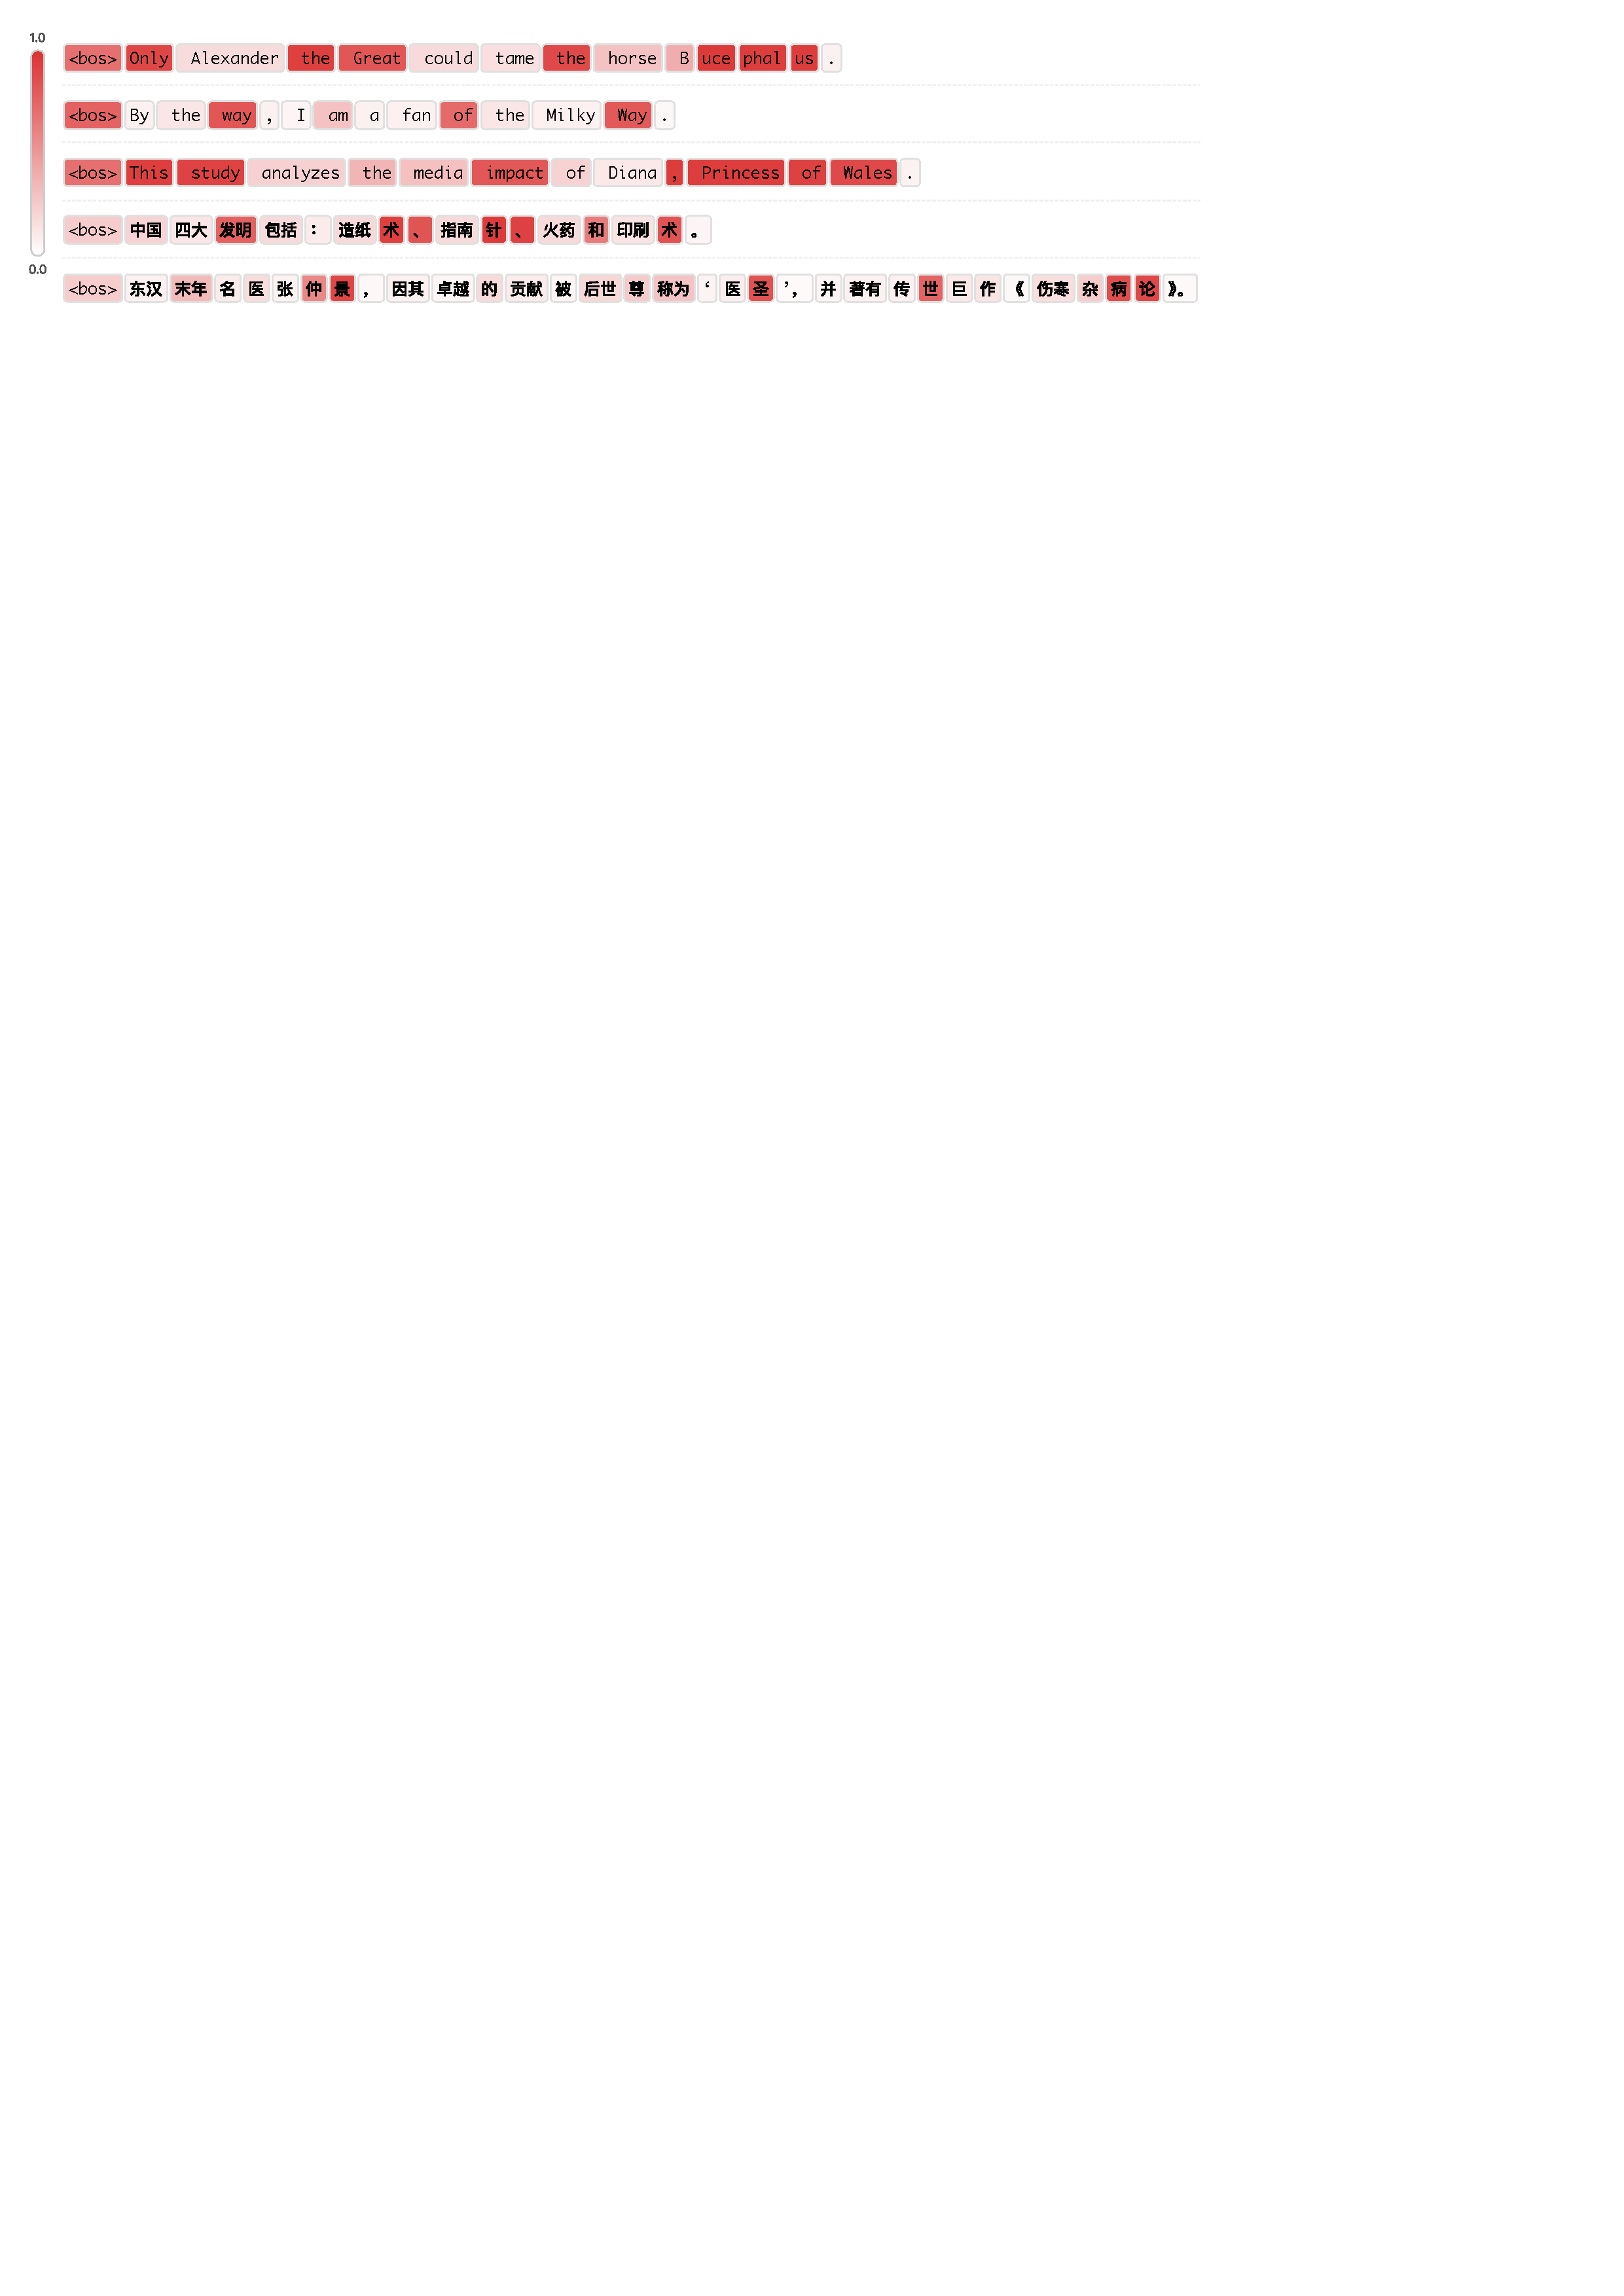
\includegraphics[width=1.0\linewidth]{figs/visualization.pdf}
    \caption{
        \textbf{Visualization of the gating mechanism of Engram.} The heatmap intensity corresponds to the magnitude of the gating scalar $\alpha_t \in [0, 1]$, where darker red indicates stronger activation. Because Engram operates on suffix $N$-grams (here $N=3$), a high activation on a specific token $x_t$ implies that the preceding tokens culminating in that token (e.g., the phrase ending at $t$) are recognized as a static pattern effectively retrieved from memory.
    }
    \label{fig:visualization}
\end{figure}